\section{Evaluation}\label{sec:eval}

We evaluate \sysname{} using a combination of testbed experiments and numerical experiments. Our evaluation centers around three key questions:

\begin{itemize}
	\item \textbf{Can \sysname{} prevent deadlock when deadlock-prone misconfiguration or network failure happens?} We considered both loop scenario and none loop scenario, and validate that \sysname{} can prevent deadlock when deadlock-prone misconfiguration or network failure happens.
	
	\item \textbf{Is \sysname{} scalable for general datacenter networks?}  For Jellyfish~\cite{jellyfish}, we calculate the  number of lossless priority classes, the total number of ACL rules and the number of ACL rules at bottleneck switch under varying network size. We found that our \sysname{} requires only 3 lossless priority classes and no more than 100 ACL rules per switch for large scale Jellyfish networks with 2,000 switches. 
	
	\item \textbf{Does \sysname{} introduce significant performance overhead?} We evaluated both throughput overhead and latency overhead of \sysname{}, and found that it does not introduce any remarkable overhead.
	
	
\end{itemize}

\begin{figure}
	\centering
	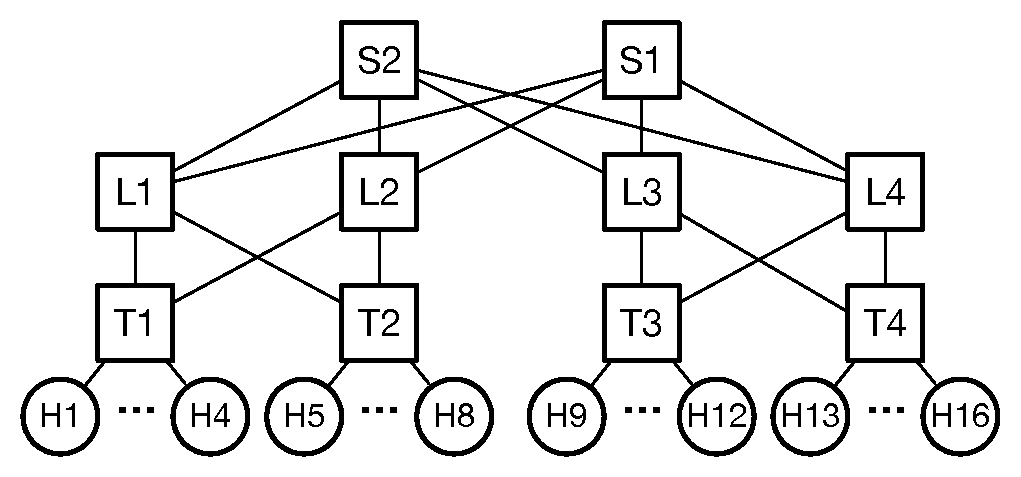
\includegraphics[width=0.45\textwidth] {figs/testbed_topo}
	\caption{Testbed Topology.}\label{fig:testbed_topo}
	
\end{figure}



\textbf{Testbed setup}: We built a small clos network as our testbed with 16 servers and 10 switches, as shown in Figure~\ref{fig:testbed_topo}. Each server is a Dell PowerEdge R730 server with a 40Gbps Mellanox ConnectX-3 Pro NIC, two 16-core Intel E5-2698 2.3GHz CPUs, 256GB memory and 
2TB hard disk. Each switch is a Arista 7060CX-32S switch with 32 100Gbps ports and 16MB packet buffer. Our switches support
PFC with at most 8 priority classes. Our ConnectX-3 Pro NICs support RoCEv2 and DCQCN protocol.


\subsection{Validation}\label{subsec:exp_validation}

\begin{figure}[t]
	%\vspace{-0.1in}
	\centering
	
	\subfloat[short for lof][] {
		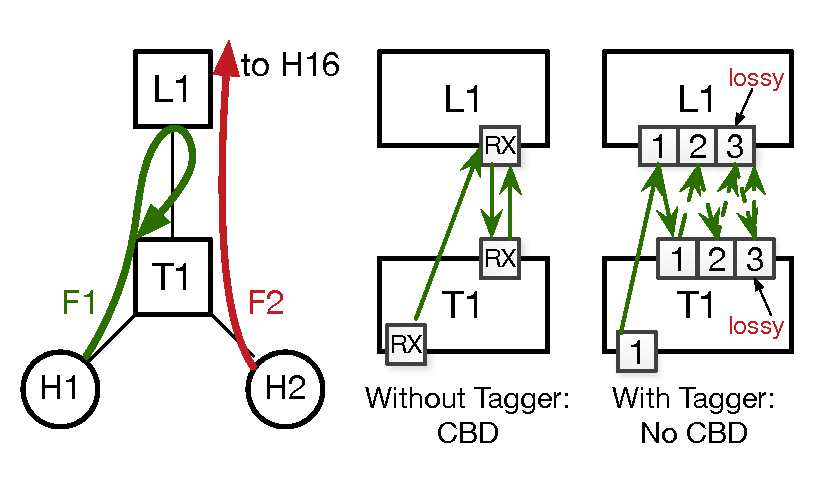
\includegraphics[width=0.2\textwidth] {figs/validation_loopcase_scenario}
	}
	\subfloat[short for lof][]{
		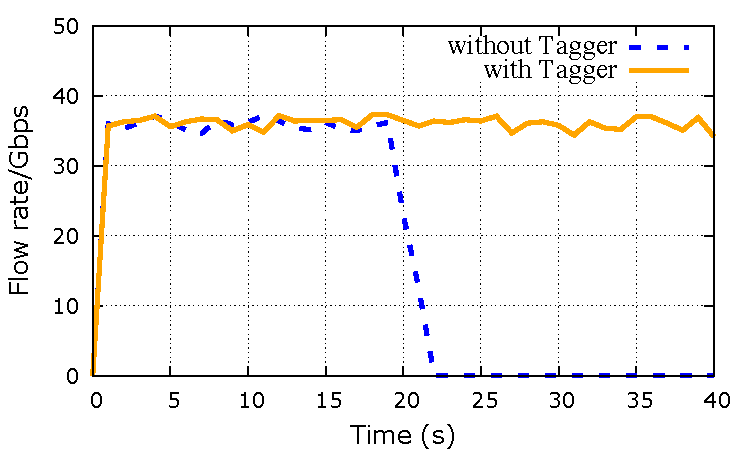
\includegraphics[width=0.3\textwidth] {figs/validation_loopcase_flowrate}
	}
	
	\caption{Loop scenario.}\label{fig:exp_validation_loop}
	
\end{figure}

\begin{figure}[t]
	%\vspace{-0.1in}
	\centering
	
	\subfloat[short for lof][] {
		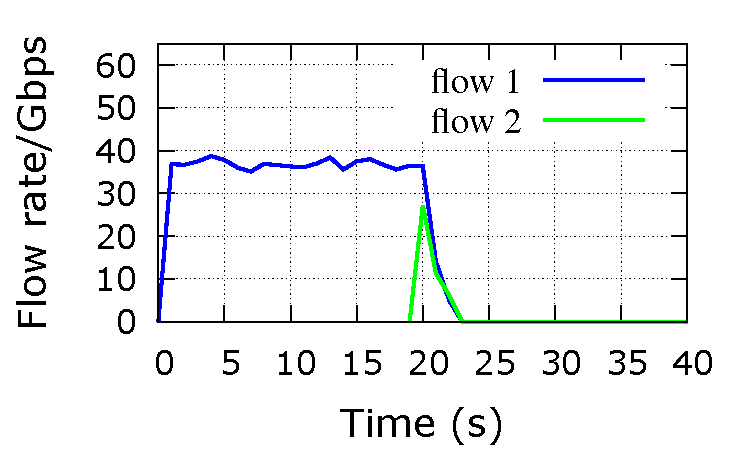
\includegraphics[width=0.25\textwidth] {figs/validation_nonloopcase_flowrate_notagger}
	}
	\subfloat[short for lof][]{
		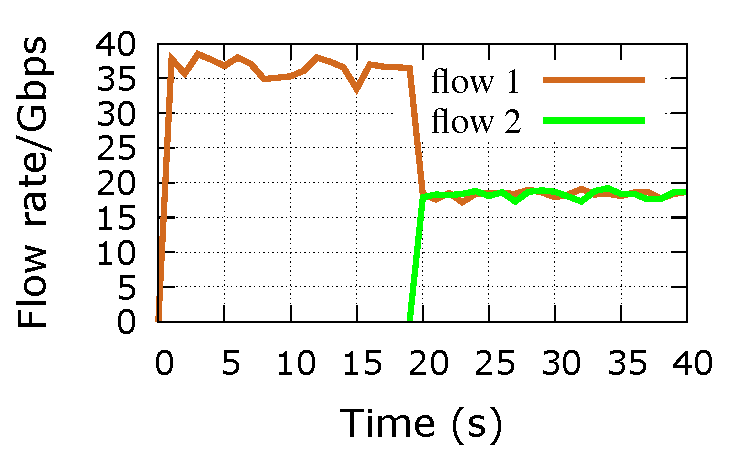
\includegraphics[width=0.25\textwidth] {figs/validation_nonloopcase_flowrate_tagger}
	}
	
	\caption{None loop scenario.}\label{fig:exp_validation_nonloop}
	
\end{figure}


In this experiment, we demonstrate that \sysname{} can prevent deadlock when there is CBD. We consider both loop scenario and none loop scenario.

\textbf{Loop scenario:} As shown in Figure~\ref{fig:exp_validation_loop}(a), we generate 2 flows across different ToRs, i.e., flow 1 from H1 to H15 and flow 2 from H2 to H16. At time = 20s, we install a bad route at L1 to let flow 1 enter a routing loop between T1 and L1. The path taken by flow 2 also traverses link T1-L1. 

In Figure~\ref{fig:exp_validation_loop}(b), we plot the rate of flow 2 with and without \sysname{}. As we can see, if \sysname{} is not applied, deadlock occurs and flow 2 is paused due to propagation of PFC PAUSE. With \sysname{}, there is no deadlock and rate of flow 2 is not affected by the routing loop.

\textbf{None loop Scenario:} we generate 2 flows to emulate the scenario shown in Figure~\ref{fig:priority_transition}(b), where two 1-bounce paths form a CBD. In this experiment, We run flow 1 at first, and let flow 2 join in at time = 20s. 

In Figure~\ref{fig:exp_validation_nonloop}(a), we plot the rate of both flows when \sysname{} is not applied. In Figure~\ref{fig:exp_validation_nonloop}(b), we plot the rate of both flows when \sysname{} is applied. As we can see,
Without \sysname{}, deadlock occurs and rate of both flows are reduced to 0. With \sysname{}, there is no deadlock and flow rate is not affected..

\subsection{Overhead}\label{subsec:exp_overhead}

\subsubsection{Resource Consumption}\label{subsec:exp_resourceconsump}

\begin{table*}[t]
	\centering
		\begin{tabular}{|r|r|r|r|r|r|}
			\hline
			Switch $\#$ &  Switch port $\#$ &  Network diameter &	\multicolumn{1}{c|}{\tabincell{c}{\text{$\#$ of lossless} \\ \text{priority classes}}}    & Total $\#$ of rules &    
			\multicolumn{1}{c|}{\tabincell{c}{\text{$\#$ of rules at} \\ \text{bottleneck switch}}}\\
			\hline
			\hline
			10 & 12 & 5 & 2 & 116 & 10 \\
			\hline
			100 & 32 & 6 & 3 & 3,794 & 37 \\
			\hline
			500 & 64 & 6 & 3 & 36,508 & 76 \\
			\hline
			1,000 & 64 & 6 & 3 & 81,136 & 88 \\
			\hline
			2,000 & 64 & 7 & 3 & 185,921 & 98 \\
			\hline
			
		\end{tabular}
	\caption{Resource consumption of Algorithm~\ref{alg:greedy} on Jellyfish at different scales.}
	\label{table:resource_consumption}
\end{table*}

In this part, we evaluate the resource consumption of our greedy algorithm (Algorithm~\ref{alg:greedy}) on Jellyfish~\cite{jellyfish} in terms of number of lossless priority classes and number of ACL rules. 

Jellyfish topology is an r-regular random graph, and has three parameters N, k and r. N is the number of switches, k is the number of ports a switch has and r is the number of ports used to connect with other switches (the
remaining k − r ports are for servers). In our experiment, we let r = k/2.
We construct the routing paths by building destination-rooted shortest-path spanning trees at all the servers.

As shown in Table~\ref{table:resource_consumption}, we measured $\#$ of lossless priority classes, total $\#$ of rules\footnote{Total $\#$ of rules to be installed in all the switches} and $\#$ of rules at bottleneck switch \footnote{ Bottleneck switch refers to the switch which has the maximum number of ACL rules to be installed.} under varying network size. 

The results in the table demonstrate our solution is scalable: In terms of the  lossless priority classes, our solution requires only 3 lossless classes for a large network of 2,000 switches.  In terms of the ACL rules to be installed, no more than 100 rules are needed to be installed at the bottleneck switch, while most commodity switches can support 1K-4K hardware ACL rules.

\subsubsection{Performance overhead}\label{subsec:exp_performanceoverhead}

\begin{figure}
	\centering
	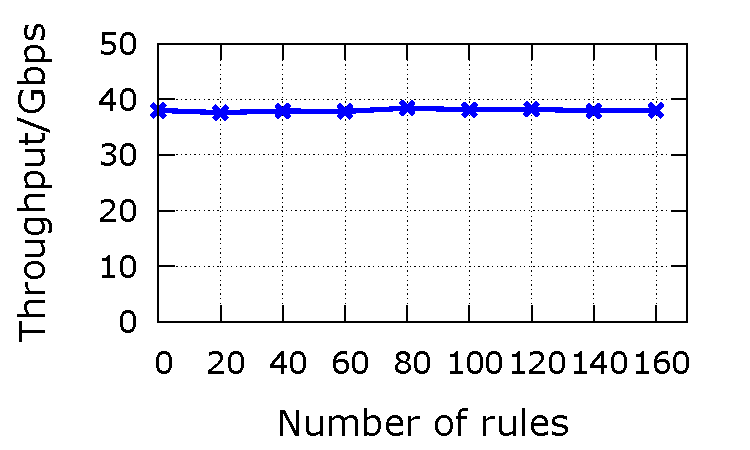
\includegraphics[width=0.45\textwidth] {figs/overhead_avgthrpt}
	\caption{Measurement of throughput overhead.}\label{fig:thrpt_overhead}
\end{figure}



\begin{table}[t]
	\centering
	\scalebox{0.9}{
	\begin{tabular}{|r|r|r|r|r|r|}
		\hline
		$\#$ of rules & Average RTT (us) &   \multicolumn{1}{c|}{\tabincell{c}{\text{50th percentile} \\ \text{RTT (us)}}}   & \multicolumn{1}{c|}{\tabincell{c}{\text{99th percentile} \\ \text{RTT (us)}}} \\
		\hline
		\hline
		10 & 77 & 81 & 104  \\
		\hline
		20 & 79 & 77 & 99  \\
		\hline
		40 & 77 & 74 & 106 \\
		\hline
		80 & 81 & 82 & 101 \\
		\hline
		160 & 75 & 77 & 104 \\
		\hline
		
	\end{tabular}
     }
	\caption{Measurement of latency overhead.}
	\label{table:latency_overhead}
\end{table}


The ACL rules \sysname{} installed are TCAM-based hardware rules. Hence it introduces little performance overhead. In this part, we evaluate the performance overhead of \sysname{} with the following two experiments.
 
 \textbf{Throughput overhead}: we generate one flow from H1 to H2, and observe its average throughput over 100 seconds under varying number of \sysname{} rules installed in T1. As shown in Figure~\ref{fig:thrpt_overhead}, the average throughput remains stable when increasing number of installed rules.

 \textbf{Latency overhead}: We install different number of \sysname{} rules in T1 and measure the RTT between H1 and H2. We repeat pinging 5,000 times and calculate average RTT, 50th percentile RTT and 99th percentile RTT, as shown in Table~\ref{table:latency_overhead}. As we can see, the number of installed rules does not have any significant impact on network latency.


%\subsection{Impact of priority reusing}\label{subsec:exp_priorityreusing}
%
%
%\begin{figure}
%	%\vspace{-0.1in}
%	\centering
%	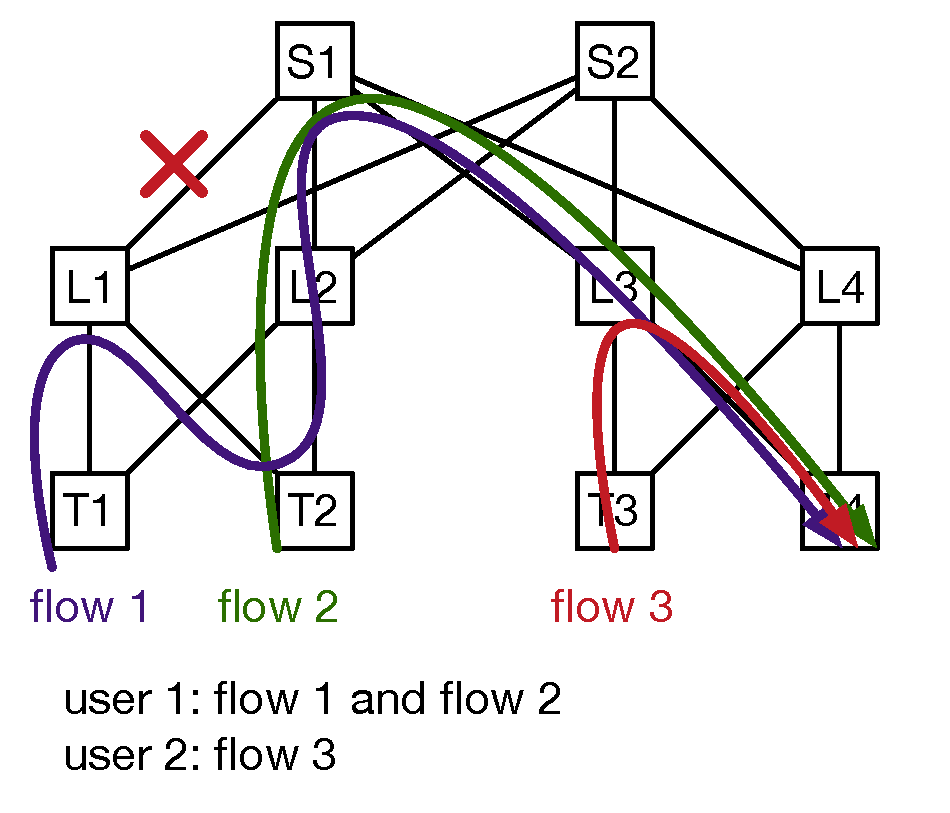
\includegraphics[width=0.45\textwidth] {figs/priorityreusing_1}
%	\caption{Scenario of priority reusing experiment.}\label{fig:exp_priorityreusing}
%	
%\end{figure}
%
%\textbf{Purpose:} demonstrate the mechanism of priority reusing will not downgrade link utilization and throughput of flows (but may introduce unfairness problem).
%
%\textbf{Scenario:} As shown in Fig.~\ref{fig:exp_priorityreusing}(a), a Clos network serves two users belonging to different application classes. For user 1, priority 1 is used for traffic following shortest paths, and priority 2 is used for traffic following 1-bounce paths. For user 2, priority 2 is used for traffic following shortest paths, and priority 1 is used for traffic following 1-bounce paths.
%
%Assuming WRR policy among different egress queues. Assuming traffic of these two users shares a bottleneck link. We create a link failure to let flow 1 of user 1 enter the second lossless space. Flow 1 then competes link bandwidth in the same egress queue with flow 3 of user 2 at the bottleneck link L3-T4. 
%
%By measuring the link utilization and throughput of all flows, we can demonstrate that link utilization of the bottleneck link and overall throughput of all flows is not downgraded, but priority reusing does cause some unfairness problem among different suers.
%
%\textbf{compared scheme:} no priority reusing among users (4 priorities are used)
%  
%\subsection{Hierarchical lossless space improves application performance}\label{subsec:exp_appperformance}
%
%\textcolor{red}{This experiment will be moved to Section 3 as an motivation experiment.}
%
%\textbf{Purpose:} demonstrate that for Clos network, applications can achieve better performance when both shortest paths and 1 bounce paths are lossless.
%
%\textbf{Scenario:} In a Clos network, we run both throughput-intensive and latency-sensitive applications. We randomly generate k failures in the network to have some of the flows follow 1-bounce paths.
%
% \textbf{compared schemes:}
% \begin{enumerate}
% 	\item both shortest paths and  1 bounce paths are lossless.
% 	\item shortest paths are lossless. 1 bounce paths are lossy.
% 	\item Only shortest paths are allowed.
% \end{enumerate}
%  
%  
  
%\subsection{Lossless transition between priority classes}\label{subsec:exp_losslesstransition}
%
%%\begin{figure}[t]
%%	%\vspace{-0.1in}
%%	\centering
%%	
%%	\subfloat[short for lof][] {
%%		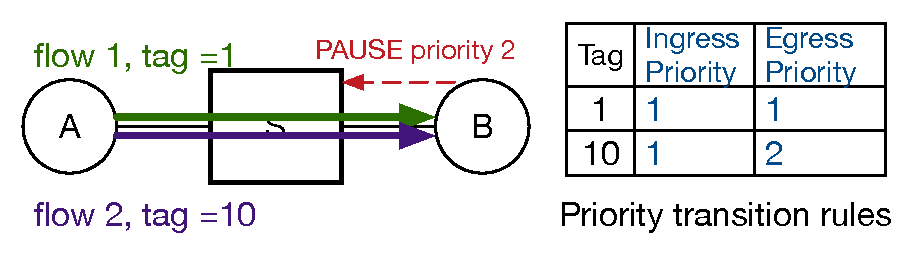
\includegraphics[width=0.43\textwidth] {figs/exp_queuetransition_1}
%%	}
%%	
%%	\vspace{-0.15in}
%%	\subfloat[short for lof][]{
%%		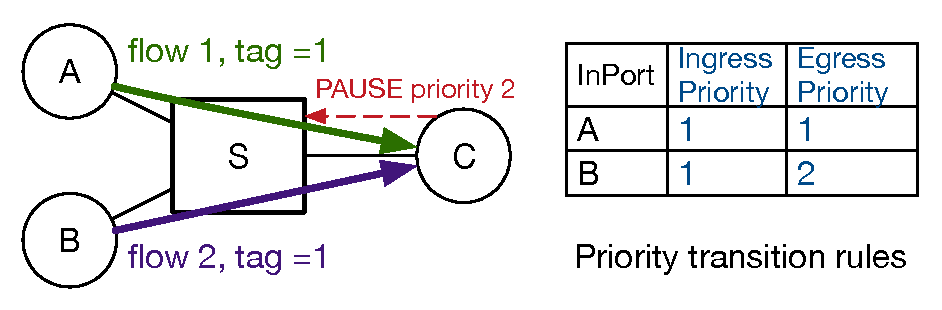
\includegraphics[width=0.43\textwidth] {figs/exp_queuetransition_2}
%%	}
%%
%%\vspace{-0.15in}
%%	\subfloat[short for lof][]{
%%	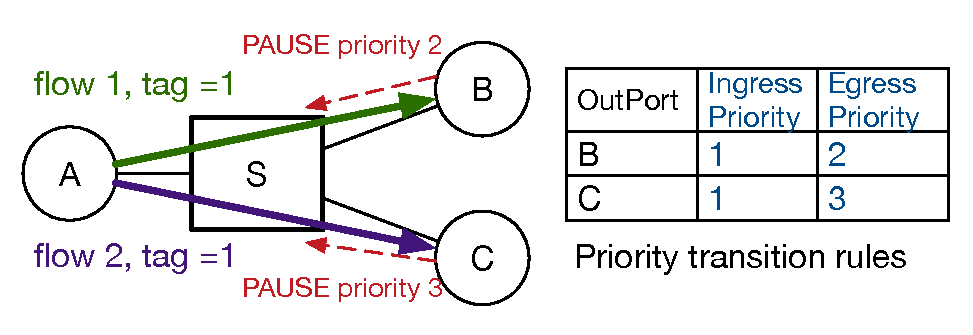
\includegraphics[width=0.43\textwidth] {figs/exp_queuetransition_3}
%%     }
%%	
%%	\caption{Experiment scenarios to demonstrate lossless transition between priority classes.}\label{fig:exp_queuetransition}
%%\end{figure}
%
%\textbf{Purpose:} demonstrate our implementation ensures lossless transition between priority classes.
%
%\textbf{Scenario-1:} As shown in Fig.~\ref{fig:exp_queuetransition}(a), by pausing priority 2 at server B, flow 2 is paused correctly without any packet loss, while flow 1 is not affected.
%
%\textbf{Scenario-2:} As shown in Fig.~\ref{fig:exp_queuetransition}(b), by pausing priority 2 at server C, flow 2 is paused correctly without any packet loss, while flow 1 is not affected.
%
%\textbf{Scenario-3:} The scenario is shown in Fig.~\ref{fig:exp_queuetransition}(c). By pausing priority 2 at server B, flow 1 is paused correctly without any packet loss. By pausing priority 3 at server C, flow 2 is paused correctly without any packet loss.
  
  
  
%   \subsection{Experiment 7: dealcok-free reconfiguration of ACL rules.}\label{subsec:exp_acloverhead}
%   
%   \textbf{Point to demonstrate:} when operator changes the topology or desired routing, we can do an online dealcok-free reconfiguration of ACL rules.
%   
%    \textcolor{red}{need a solution to do dealcok-free reconfiguration of ACL rules at first.}
    
    
    % \subsection{Experiment 2: CBD probability}\label{subsec:exp_CBDprobability}
    % 
    % \textbf{Point to demonstrate:} it is easy for a network to have CBD.
    % 
    % \textbf{Setup:} for Fattree, we randomly generate k failures or misconfiguration, and evaluate whether CBD is created.
    % 
    %  for BCube and Jellyfish, we calculate the default lossless routing by randomly choosing m shortest paths between each node pair. And then we check whether the output routing includes CBD.
  
  
  %\begin{table}[t]
  %	\centering
  %	\begin{tabular}{|r|r|}
  %		  tag & ingress queue  \\
  %		\hline
  %		\hline
  %		0 & 0 \\
  %		\hline
  %		1 & 1 \\
  %		\hline
  %		2 & 2 \\
  %		\hline
  %		3 & 3 \\
  %		\hline
  %		others & lossy \\
  %		\hline
  %	\end{tabular}
  %	\caption{Ingress queueing rules under Algorithm 1.}
  %	\label{table:tagging_table}
  %\end{table}
  %
  %\begin{table}[t]
  %	\centering
  %	\begin{tabular}{|r|r|}
  %		newtag & egress queue  \\
  %		\hline
  %		\hline
  %		1 & 1 \\
  %		\hline
  %		2 & 2 \\
  %		\hline
  %		3 & 3 \\
  %		\hline
  %		others & lossy \\
  %		\hline
  %	\end{tabular}
  %	\caption{Egress queueing rules under Algorithm 1.}
  %	\label{table:tagging_table}
  %\end{table}
  
  
  
  %\begin{table}[t]
  %	\centering
  %	\begin{tabular}{|r|r|}
  %		tag & ingress queue  \\
  %		\hline
  %		\hline
  %		0 & 0 \\
  %		\hline
  %		1 & 1 \\
  %		\hline
  %		others & lossy \\
  %		\hline
  %	\end{tabular}
  %	\caption{Ingress queueing rules under Algorithm 3.}
  %	\label{table:tagging_table}
  %\end{table}
  %
  %\begin{table}[t]
  %	\centering
  %	\begin{tabular}{|r|r|}
  %		newtag & egress queue  \\
  %		\hline
  %		\hline
  %		0 & 0 \\
  %		\hline
  %		1 & 1 \\
  %		\hline
  %		others & lossy \\
  %		\hline
  %	\end{tabular}
  %	\caption{Egress queueing rules under Algorithm 3.}
  %	\label{table:tagging_table}
  %\end{table}
  
  